\section{Rækkeudviklinger} \label{mat:sec:raekker}
Rækkeudviklinger er navnet på en teknik man bruger gentagne gange i fysik. En række er en sum efter et bestemt system, hvilket eksempelvis kunne være summen af heltal mindre end eller lig med 100,
%
\begin{align}
    \sum_{n=0}^{100}n = 0 + 1 + 2 + ... 100 = 5050.
\end{align}
%
Ideen med en rækkeudvikling er, at man i fysik ofte støder på ligninger, der er svære at løse eller slet ikke har en analytisk løsning. En almindelig tilgang er så at finde en approksimativ løsning, som man så systematisk kan forbedre. Lad os se på et eksempel, for at forstå hvad det handler om.

\subsubsection{Eksempel I}
Tre personer har købt en gave til en fjerde person til \SI{292}{kr}. og vil dele udegiften ligeligt. Prisen, de hver skal betale, kaldes $p$ og den er
%
\begin{align}
    p = \frac{292}{3}\,\si{kr}.
\end{align}
%
Det er ikke en simpel, velkendt brøk, og kan derfor tage lidt tid, at få reduceret i hovedet. Vi kan dog bruge tanken om rækkeudviklinger, til at gøre dette lettere for os selv. Først bemærkes det at 292 er meget større end 3, hvorfor man som første approksimation kan runde 292 op til 300.
%
\begin{align}
    \frac{292}{3}\,\si{kr}. \approx \frac{300}{3}\,\si{kr}. = \SI{100}{kr}. = x_1
\end{align}
%
Denne simpleste approksimation kalder vi $x_1$. Vi rundede op ved at lægge 8 til, men det største heltal mindre end 8, som 3 går op i er 6. Derfor kan vi forbedre approksimationen af $p$ ved at lægge
%
\begin{align}
    x_2 = -\frac{6}{3}\,\si{kr}. = -\SI{2}{kr}.
\end{align}
%
til $x_1$, således at den anden approksimation af prisen er
%
\begin{align}
    p \approx x_1 + x_2 = \SI{100}{kr}. + \left(-\SI{2}{kr}.\right) = \SI{98}{kr}.
\end{align}
%
Det sidste vi nu mangler at tage højde for, er ´resten' fra divisionen af 8 med 3. Det vil sige at
%
\begin{align}
    x_3 = -\frac{2}{3}\,\si{kr}. = -0,66...\,\si{kr}.
\end{align}
%
Den pris de tre personer hver skal betale er således
%
\begin{align}
    p = x_1 + x_2 + x_3 = \sum_{n=1}^3 x_n = \SI{100}{kr}. + \left(-\SI{2}{kr}.\right) + \left(-0,66...\,\si{kr}.\right) = 97,66...\,\si{kr}.
\end{align}
%
Pointen med eksemplet er, at man kunne lave et ´svært' regnestykke om til en serie af lettere regnestykker, som uden problemer kunne klares ved hovedregning. Der hvor denne tankegang bliver smart, er når problemet bliver svært eller umuligt at løse.

\subsubsection{Eksempel II}
I \cref{mat:sec:diff} blev Eulers tal defineret som værende det tal, der har egenskaben at $\nicefrac{\dd{e^x}}{\dd{x}} = e^x$. En ting er at have en definition af tallet, men det er ikke meget værd, hvis man ikke har en måde, hvorpå man kan regne ud, hvilken værdi dette tal har. Det viser sig at $e$ er et irrationelt tal, hvilket betyder, at det ikke kan skrives som en brøk. Det viser sig Eulers tal kan rækkeudvikles -- man kan skrive som en uendelig sum,
%
\begin{align} \label{mat:eq:e-raekke}
    e = \frac{1}{0!} + \frac{1}{1!} + \frac{1}{2!} + ... = \sum_{n=0}^\infty \frac{1}{n!},
\end{align}
%
hvor det bemærkes at $0! = 1$. Ud fra definitionen af fakultet, \cref{mat:eq:fakultet}, kan det virke underligt, men det er ikke noget, vi vil bevise her. En uendelig sum kaldes også en uendelig række eller blot en række og man siger derfor at \cref{mat:eq:e-raekke} er en rækkeudvikling af Eulers tal\footnote{Den opmærksomme læser spørger måske sig selv om hvordan det kan passe, at man ved at lægge uendeligt mange brøkker sammen, kan få et tal, der ikke kan skrives ved hjælp af brøker? Svaret er, at det tal man får, når man evaluerer den uendelige række, er uendeligt tæt på $e$, hvorfor man siger at rækken konvergerer mod $e$. Lighedstegnet betyder i dette tilfælde ``uendeligt tæt på'', hvilket i fysik siges, at være det samme som ``lig med''.}. Eulers tal kan nu approksimeres af en computer, ved at beregne summen af de første $N$ led i rækken. Gør man det, finder man ud af, at tallet ikke ændrer sig ret meget efter de første ca. 10 led. Har man i laboratoriet målt noget til en præcision på 2 betydende cifre, så er det rigeligt at have $e$ med eksempelvis 5 betydende cifre, hvilket man får med de første 10 led. En rækkeudvikling kan derfor forstås som en approksimation, der bliver bedre desto flere led vi tager med, hvilket vi også så i eksempel I. \\

I fysik beskriver man ofte fysiske størrelser med en funktion, og vi vil derfor udvide tanken om rækkeudviklinger til netop funktioner. % I fysikken prøver man generelt at give en så præcis beskrivelse af virkeligheden som muligt, men i mange tilfælde kan det ikke lade sig gøre at løse et givet problem eksakt. Derfor må man tit vælge enten at kigge på specialtilfælde af problemet, der kan løses, eller at finde en approksimativ løsning til problemet, som kan give noget information omkring, hvordan ens fysiske system opfører sig. Et eksempel på dette kunne fx. være et pendul, hvor man tit kan antage, at vinklerne ved udsving er små, hvilket giver en betydeligt simplere bevægelsesligning for pendulet. 
Et vigtigt redskab til dette formål er \emph{Taylorapproksimationer}, som er en måde at approksimere en given funktion $f(x)$ omkring et bestemt punkt $x=a$, vha. en sum af polynomier $1,x,x^2,\ldots$ I denne forbindelse defineres det, der kaldes et \emph{Taylorpolynomium}:
%
\begin{equation}
\label{mat:eq:Taylor_pol}
T_N(x) = \sum\limits_{n = 0}^{N} \frac{f^{(n)}(a)}{n!} (x-a)^n = f(a) + \frac{f^{(1)}(a)}{1!} (x-a)  + ... + \frac{f^{(N)}(a)}{N!}(x-a)^N  \ .
\end{equation}
%
Her skal $f^{(n)}(a)$ læses som funktionen $f(x)$ differentieret $n$ gange, og derefter evalueret i punktet $a$. Dette skrives også nogle gange med en anden notation, der minder mere om den, der er brugt i afsnittet om differentialregning, men som er lidt tungere at skrive.
\begin{equation} \label{mat:eq:diff_eval}
f^{(n)}(a) = \left.\dv[n]{f}{x}\right|_ {x=a} \; .
\end{equation}
Når en funktion, $f(x)$, approksimeres med et Taylorpolynomium, $T_N(x)$, omkring punktet $x=a$, skriver man, at $f(x) \approx T_N(x)$ for $x \approx a$, for at indikere at $f(x)$ er cirka lig med $T_N(x)$, når $x$ er cirka lig med $a$.\\

%
\begin{figure}[t]
	\centering
	\begin{subfigure}{.475\textwidth}
	    \centering
    	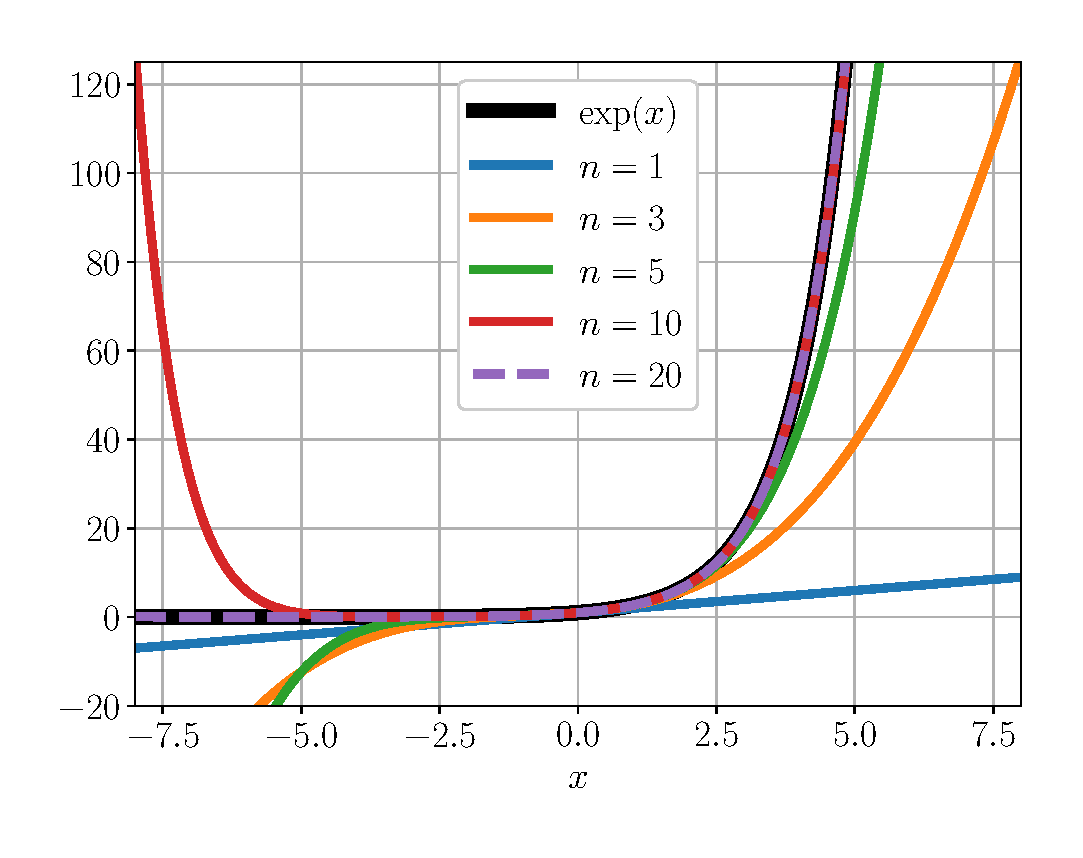
\includegraphics[width=\columnwidth]{Matematik/matfig/taylor.eps}
    	\caption{Lineær andenakse.}
    	\label{mat:eq:taylor_lin}
    \end{subfigure}
    %
    \hfill
    %
	\begin{subfigure}{.475\textwidth}
	    \centering
    	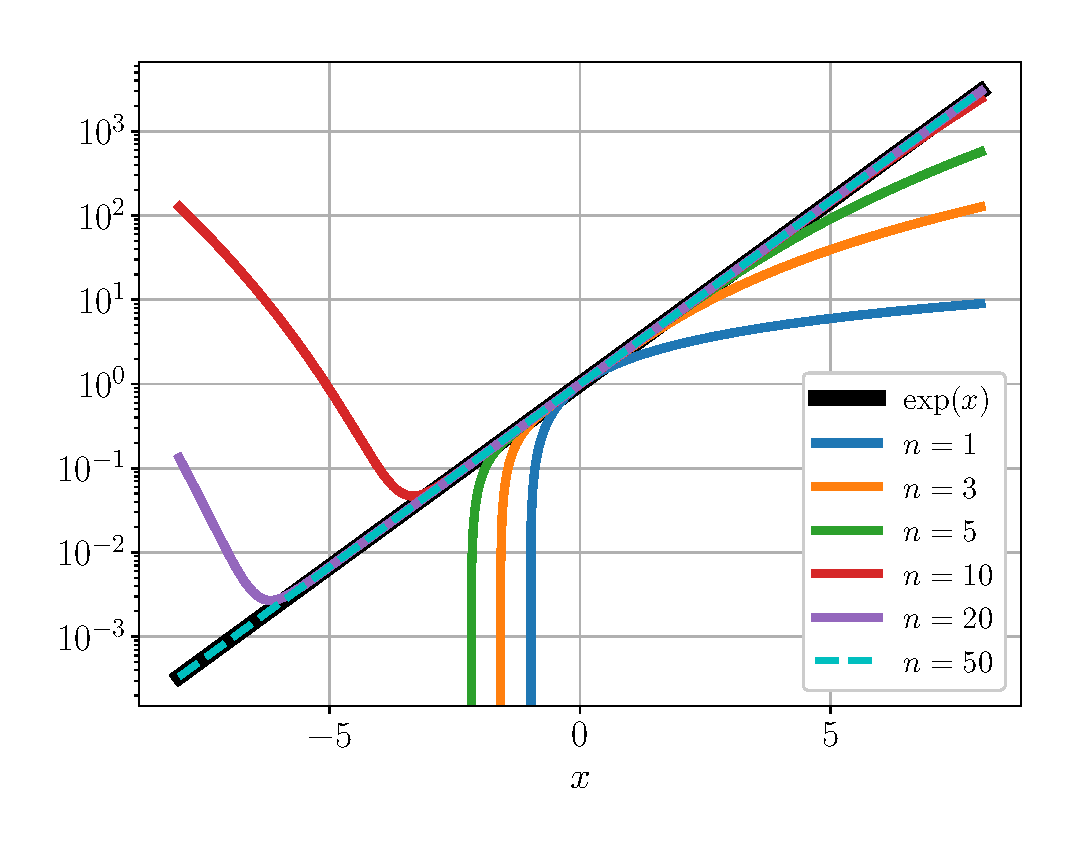
\includegraphics[width=\columnwidth]{Matematik/matfig/taylor_log.eps}
    	\caption{Logaritmisk andenakse.}
    	\label{mat:eq:taylor_log}
    \end{subfigure}
	\caption{Taylorpolynomierne $T_1(x), \, T_3(x), \, T_5(x), \,T_{10}(x), \, T_{20}(x)$ for $f(x) = e^x$ omkring punktet $a=0$. Eksemplet illustrerer hvordan en Taylorapproksimation bliver bedre og bedre, jo flere led der tages med. I \cref{mat:eq:taylor_log} er $T_{50}(x)$ tilføjet, da man her kan se forskel på den og $T_{20}(x)$. Det vigtige i figurerne er, at jo større $n$ bliver, desto tættere kommer $T_n(x)$ på $f(x)$.}
	\label{mat:fig:Taylorseries_figure}
\end{figure}
%
Ved første øjekast er det måske svært at gennemskue, hvad \cref{mat:eq:Taylor_pol} har med at approksimere en funktion at gøre, så vi vil derfor undersøge hvorfor formlen ser ud, som den gør. Lad os derfor kigge på funktionen $f(x) = e^x$, og prøve at approksimere den omkring punktet $a = 0$. Den simpleste approksimation man kan lave, er at approksimere $f(x)$ som en konstant. Da vi gerne vil beskrive funktionen omkring punktet $a=0$, er den bedste konstante approksimation $f(x)$ selv evalueret i punktet $a$. Altså
$$f(x) \approx f(a) = e^a = e^0 = 1$$
Det næste man kan gøre er da, at tilføje en hældning til vores approksimation. Det bedste valg er hældningen af $f(x)$ selv i punktet $a$. Den er
$$f^{(1)}(a) = \left. \dv{f(x)}{x} \right|_{x=a} = \left. \dv{}{x}e^x \right|_{x=a} \left. = e^x \right|_{x=a} = e^a = 1$$
Det giver den nye approksimation af $f(x)$
$$f(x) \approx 1 + x \ ,$$
der netop giver den eksakte værdi for både funktionsværdienværdien og hældningen af $f(x)$ i punktet $x=a$. Man kan så også tilføje en krumning (ændringen i hældningen) til vores approksimation. Igen er det bedste valg krumningen af $f(x)$ i punktet $a$, hvilket giver
$$f^{(2)}(a) = \left. \dv[2]{f(x)}{x} \right|_{x=a} = \left. \dv[2]{}{x} e^x \right|_{x=a} \left. e^x \right|_{x=a} = e^a = 1$$
Den nye approksimation bliver da
$$f(x) \approx 1 +  x + \frac{1}{2} x^2 \ ,$$
hvor $\nicefrac{1}{2}$ er taget med for at sikre at krumningen af approksimation er lig med krumningen af $f(x)$ i punktet $a$, da den afledede af $x^2$ er $2x$. At dette faktisk er tilfældet kan vises ved en hurtig beregning
%
\begin{equation*}
\left. \dv[2]{}{x} \left(1+x+\frac{1}{2}x^2\right) \right|_{x=a} = \left. \dv{}{x} \left(1+x\right) \right|_{x=a} = \left. 1 \right|_{x=a} = 1 = f^{(2)}(a) \; .
\end{equation*}
%
\begin{table}[t]
	\centering
	\caption{Taylorpolynomier for forskellige funktioner omkring punktet $a=0$.}
	\label{mat:tab:Taylorseries_table}
	\bgroup
	\def\arraystretch{2}
	\begin{tabular}{|c|c|c|c|}
		\hline
		\textbf{Funktioner}   & $e^x$ & $\cos(x)$ & $\sin(x)$  \\ 
		\hline
		\textbf{Taylorpolynomier} & $\sum\limits_{n = 0}^{N} \dfrac{x^n}{n!}$ & $\sum\limits_{n=0}^{N} (-1)^n \dfrac{x^{2n}}{(2n)!} $ & $\sum\limits_{n=0}^{N} (-1)^n \dfrac{x^{2n+1}}{(2n+1)!}$  \\ \hline
	\end{tabular}
	\egroup
\end{table}
%
%
Ideen herfra er da blot at tilføje flere og flere led, så den flere og flere gange differentierede af $f(x)$ og approksimationen er lig med hinanden i punktet $a$. Ideen er også illustreret på \cref{mat:fig:Taylorseries_figure}, hvor approksimationen er vist med flere og flere led i summen.  I \cref{mat:eq:taylor_log} ses \cref{mat:eq:taylor_lin} med logaritmisk andenakse, der er den naturlige måde at tegne eksponentialfunktioner på, da de her bliver lineære. Dette gør også, at vi nu kan se forskel på $T_{20}(x)$ og $T_{50}(x)$, hvorfor den sidste er taget med. Faktisk er Taylorapproksimationen så god at Taylorrækken $T_\infty(x) = f(x)$ for de fleste funktioner og idéen er derfor den samme som med rækkeudviklingen af Eulers tal og prisen $p$ i de foregående eksempler. Vi har samlet Taylorpolynomierne for nogle af de mest almindelige funktioner omkring $a = 0$ i tabel \ref{mat:tab:Taylorseries_table}. Tanken med Taylorrækker kan tænkes som følgende: hvis blot man zoomer langt nok ind på et punkt på grafen for en funktion, så ligner funktionen en ret linje så meget, at vi næsten ikke kan se forskel. Zoomer man lidt længere ud, så ligner funktionen et andengradspolynomium, osv. Ideen med rækkeudviklinger af funktioner er faktisk mere generel end Taylorrækker, hvor man lægger polynomier med passende koefficienter sammen. Man kan også vælge at bruge sinus- og cosinusfunktion med forskellige vinkelfrekvenser, hvorved man får en såkaldt Fourierrække, hvilket der gås i dybden med i \cref{sec:fysmat}.

\subsection{Eksempel III}
Konceptet rækkeudvikling kan bruges til at opnå en større forståelse for vands varmekapacitet. I et almindeligt forsøg varmes vand op til en bestemt temperatur, og ifølge teorien er den energi opvarmningen kræver, givet ved den empiriske sammenhæng\footnote{En empirisk sammenhæng er en sammenhæng, der er fundet gennem eksperimenter og ikke teoretisk udledt.}
%
\begin{align} \label{mat:eq:cv}
    \Delta E = mc_v\Delta T,
\end{align}
%
hvor $m$ er massen af vandet, $c_v$ er vands varmekapacitet, $\Delta T$ er ændringen i temperatur og $\Delta E$ er den tilførte energi. Kigger man i en databog, ser man dog at $c_v$ er temperaturafhængig -- den har forskellige værdier ved forskellige temperaturer. Da eksperimenter viser at $\Delta E$ og $\Delta T$ hænger sammen, så eksisterer der en Taylorrække, der beskriver denne sammenhæng
%
\begin{align} \label{mat:eq:cv_taylor}
    \Delta E = m\sum_{n=1}^\infty \frac{c_v^{(n)}}{n!}\left(\Delta T\right)^n,
\end{align}
%
hvor $c_v^{(n)}$ er varmekapaciteten til $n$'te orden. Her bruges ordet orden til at referere til det led i summen, der har $\Delta T$ i den antydede potens -- $n$'te orden er altså det led, der indeholder $\left(\Delta T\right)^n$. Det viser sig, at \cref{mat:eq:cv} passer ganske fint til eksperimenter, men at $c_v$ ændrer sig en smule med temperaturen. Fortolkningen af dette er, at $c_v^{(1)} \gg c_v^{(n)}$ for $n \geq 2$, hvilket læses som $c_v^{(1)}$ er meget større end $c_v^{(n)}$ for $n \geq 2$, hvorfor fejlen, man laver, ved at bruge \cref{mat:eq:cv} i stedet for \cref{mat:eq:cv_taylor} er så lille, at det i mange sammenhænge ikke betyder noget -- eksempelvis er 4. betydende ciffer ligemeget, hvis man kun har målt med to betydende cifre. \\
Man ser samme fænomen med brydningsindekset af lys i forskellige materialer. Der eksisterer krystaller, som kan fordoble frekvensen af lys, kaldet frekvensfordoblende krystaller\footnote{Faktisk er det muligt at have krystaller, der giver lys med den $n$-dobbelte frekvens, hvilket kaldes harmonisk generation, som er meget vigtigt i eksperimenter, der kræver højenergilasere. Specifikt kaldes det 2. harmonisk generation, det der foregår i frekvensfordoblende krystaller.}, men også at nogle lasere kan fokuseres af luft, hvilket giver så høj en intensitet, at laseren river elektronerne væk fra luftmolekylerne, hvilket skaber en plasma.